\section{Versuchsaufbau und Durchführung}

\begin{figure}[h]
\centering
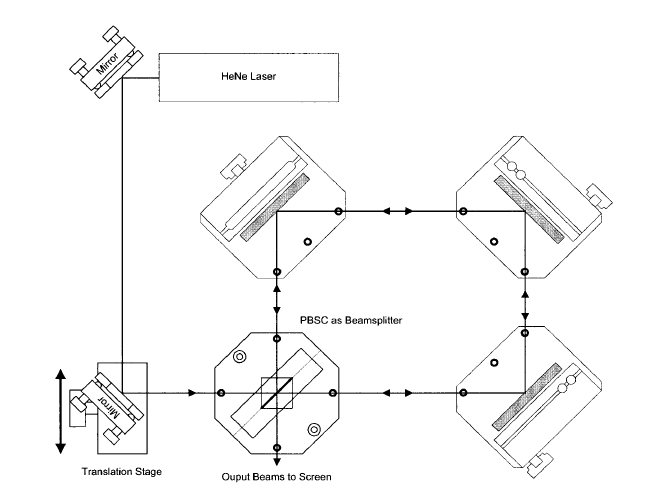
\includegraphics[scale=0.8]{./Interferometrie/img/aufbau.png}
\caption{Schematischer Aufbau der Versuchsapparatur [1]}
\label{aufbau}
\end{figure}


In diesem Versuch wird ein Sagnac-Interferometer benutzt. Der Aufbau ist in Abbildung ?? schematisch dargestellt.

\subsection{Justage}
Um das Interferometer korrekt zu Justieren, werden Plätchen welche über ein Loch verfügen, in den Strahlengang an den Positionen 1-9 positioniert. Durch den Stellschrauben an den Spigeln wird der Strahl
so eingestellt, das er durch das Loch der Justageplätchen verläuft. Sind alle Spiegel justiertm, sollen die beiden gegeläufigen Strahlen auf den Spiegeln übereinander liegen.
Es ist darauf zu achten, dass der Strahl den Optiktisch nicht verlässt.


\subsection{Messung des Kontrastes}
Um den Kontrast zu messen, wird der Doppelglashalter zwischen dem PBCS und den Spiegel $M_C$ positioniert. Danach wird der Polarisator vor dem Interferometer
von 0 bis 180 Grad gedreht. Für jede eingestellte Position wird durch Drehung des Doppelglashalters die maximale und minimale Intensität gesucht.
Die Position mit dem maximalen Kontrast wird für die folgenden Messungen eingestellt.

\subsection{Messung des Brechungsindex der Glasplatte}
Die Messungen des Brechungsindex von Glas und Luft basieren auf einer Nullmessung. Es werden nach dem Ausgang des Intferometers ein zweiter PBSC positioniert und zwei Photodioden.
Beide Photodioden werden ein einen Zähler angeschlossen, welcher Nulldruchgänge der Intensitätsdifferenz der beiden Photodioden Zählt. Der Doppelglashalter wird 
in 2 Grad Schritten von 0 Grad auf 8 Grad gedreht und die Nulldurchgänge in Abhängigkeit des Auslenkungswinkels notiert.

\subsection{Messung des Brechungsindex von Luft}
Der Doppelglashalter wird entfernt, zwischen den PBSC und dem Spiegel $M_A$ wird eine Vakuumkammer positioniert. Diese Kammer wird evakuiert und in 50 mBar Schritten
mit Sauerstoff geflutet, bis der Atmosphärendruch erreicht ist. Es werden wieder die Nulldruchläufe der Intensitätsdifferenz in Abhängigkeit des
Drucks in der Kammer gemessen.
